% !TEX root = % !TEX root = /Users/nai1ka/Projects/PerfX/Thesis/thesis.tex
\chapter{Evaluation and Discussion}
\label{chap:eval}

This chapter evaluates the performance monitoring system presented in Chapters~\ref{chap:met} and~\ref{chap:impl}. The evaluation addresses three research questions: how much overhead the SDK adds to a host application, how the regression detection pipeline identifies regressions introduced by application updates, and how accurately it does so. Section~\ref{sec:eval_setup} describes the validation setup. Section~\ref{sec:eval_overhead} reports the overhead introduced by the SDK. Section~\ref{sec:eval_accuracy} explains why the validity of the collected metrics rests on the platform APIs. Section~\ref{sec:eval_regression} evaluates the regression detection pipeline using injected regressions. Section~\ref{sec:eval_discussion} interprets the results in relation to the research questions, and Section~\ref{sec:eval_limitations} discusses the limitations of the evaluation.

\section{Validation Setup}
\label{sec:eval_setup}

The evaluation was divided into two parts: a measurement of the overhead added by the SDK (Section~\ref{sec:eval_overhead}), and an evaluation of the regression detection pipeline using injected regressions (Section~\ref{sec:eval_regression}).

\subsection{Test Devices}

The experiments were carried out on one physical Android device and three emulator instances, each configured with a different amount of RAM and a different number of CPU cores, so that the results cover all three performance cohorts defined in Section~\ref{sec:detection}. Table~\ref{tab:eval_devices} lists each device together with its hardware characteristics, its Android version, and the cohort assigned by the backend.

\begin{table}[htbp]
    \centering
    \caption{Test Devices Used in the Evaluation}
    \label{tab:eval_devices}
    \begin{tabular}{lcccc}
        \toprule
        Device                   & RAM (GB) & CPU cores & Android version & Cohort \\
        \midrule
        Emulator (Low cohort)    & 2        & 2         & 11              & Low    \\
        Emulator (Medium cohort) & 4        & 4         & 13              & Medium \\
        Xiaomi Redmi Note 9 Pro  & 6        & 8         & 15              & Medium \\
        Emulator (High cohort)   & 8        & 4         & 14              & High   \\
        \bottomrule
    \end{tabular}
\end{table}

\subsection{Test Application}

Two separate applications were used across the evaluation, each serving a different purpose.

The overhead experiments used Cheddar~\cite{cheddar}, an open-source Android client for the Hacker News website. It represents a realistic application workload, combining network requests, list rendering, and in-app navigation.

The regression detection experiments used a dedicated demo application developed as part of this project. It contains three screens that exercise different metrics, covering three regression types: increased CPU load, a memory leak, and UI thread blocking. Each experiment compared two builds of the application assigned different version codes, so the detector treated them as consecutive releases.

\section{SDK Overhead Evaluation}
\label{sec:eval_overhead}
SDK overhead was measured by running the same scenario on Cheddar in two configurations: with the SDK enabled and without it. CPU usage and memory usage were recorded during the 90-second run, and cold-start time was measured separately as the mean of ten launches. Table~\ref{tab:eval_overhead} and Table~\ref{tab:eval_startup} report the results for each test device.

\begin{table}[htbp]
    \centering
    \caption{SDK Overhead Measured on the Test Devices}
    \label{tab:eval_overhead}
    \resizebox{\textwidth}{!}{%
        \begin{tabular}{lcccccc}
            \toprule
            \multirow{2}{*}{Device}  & \multicolumn{3}{c}{CPU usage (\%)} & \multicolumn{3}{c}{Memory (MB)}                                                \\
            \cmidrule(lr){2-4} \cmidrule(lr){5-7}
                                     & Without SDK                        & With SDK                        & Overhead & Without SDK & With SDK & Overhead \\
            \midrule
            Xiaomi Redmi Note 9 Pro  & 94.6                               & 95.4                            & +0.8     & 220.1       & 222.0    & +1.9     \\
            Emulator (Low cohort)    & 39.9                               & 44.4                            & +4.5     & 149.8       & 153.5    & +3.7     \\
            Emulator (Medium cohort) & 19.6                               & 24.8                            & +5.2     & 131.1       & 136.2    & +5.1     \\
            Emulator (High cohort)   & 32.2                               & 33.9                            & +1.8     & 131.4       & 136.7    & +5.4     \\
            \bottomrule
        \end{tabular}%
    }
\end{table}

\begin{table}[htbp]
    \centering
    \small
    \caption{Cold-Start Time Overhead Measured on the Test Devices (mean of ten launches)}
    \label{tab:eval_startup}
    \begin{tabular}{lcccc}
        \toprule
        Device                   & Without SDK (ms) & With SDK (ms) & Overhead (ms) & Overhead (\%) \\
        \midrule
        Xiaomi Redmi Note 9 Pro  & 1484             & 1559          & +75           & +5.1          \\
        Emulator (Low cohort)    & 1081             & 1152          & +71           & +6.6          \\
        Emulator (Medium cohort) & 609              & 677           & +68           & +11.2         \\
        Emulator (High cohort)   & 664              & 693           & +29           & +4.4          \\
        \bottomrule
    \end{tabular}
\end{table}

On the physical Redmi Note 9 Pro, the SDK added 0.8 percentage points of CPU usage and 1.9~MB of resident memory during the 90~second scrolling scenario. The cold-start overhead was 75~ms on average, a one-time cost paid at each process launch. The CPU values can exceed 100~\% because they aggregate process time across all eight cores. The baseline of approximately 95~\% reflects a multi-core workload, not a saturated single core.

On the emulators the CPU overhead was noticeably higher in absolute terms: 4.5 percentage points on the Low-cohort emulator, 5.2 on the Medium-cohort emulator, and 1.8 on the High-cohort emulator. This is expected because the baseline CPU activity on emulators is much lower than on the physical device, so the SDK's background threads and periodic sampling make up a larger share of the total. The memory overhead was more consistent across all four devices, ranging from 1.9~MB on the physical device to 5.4~MB on the High-cohort emulator. Cold-start overhead was similar in absolute terms across all devices, between 29~ms and 75~ms.

Figure~\ref{fig:overhead_summary} shows the per-device overhead charts produced by the measurement notebook.

\begin{figure}[H]
    \centering
    \begin{subfigure}[b]{0.48\textwidth}
        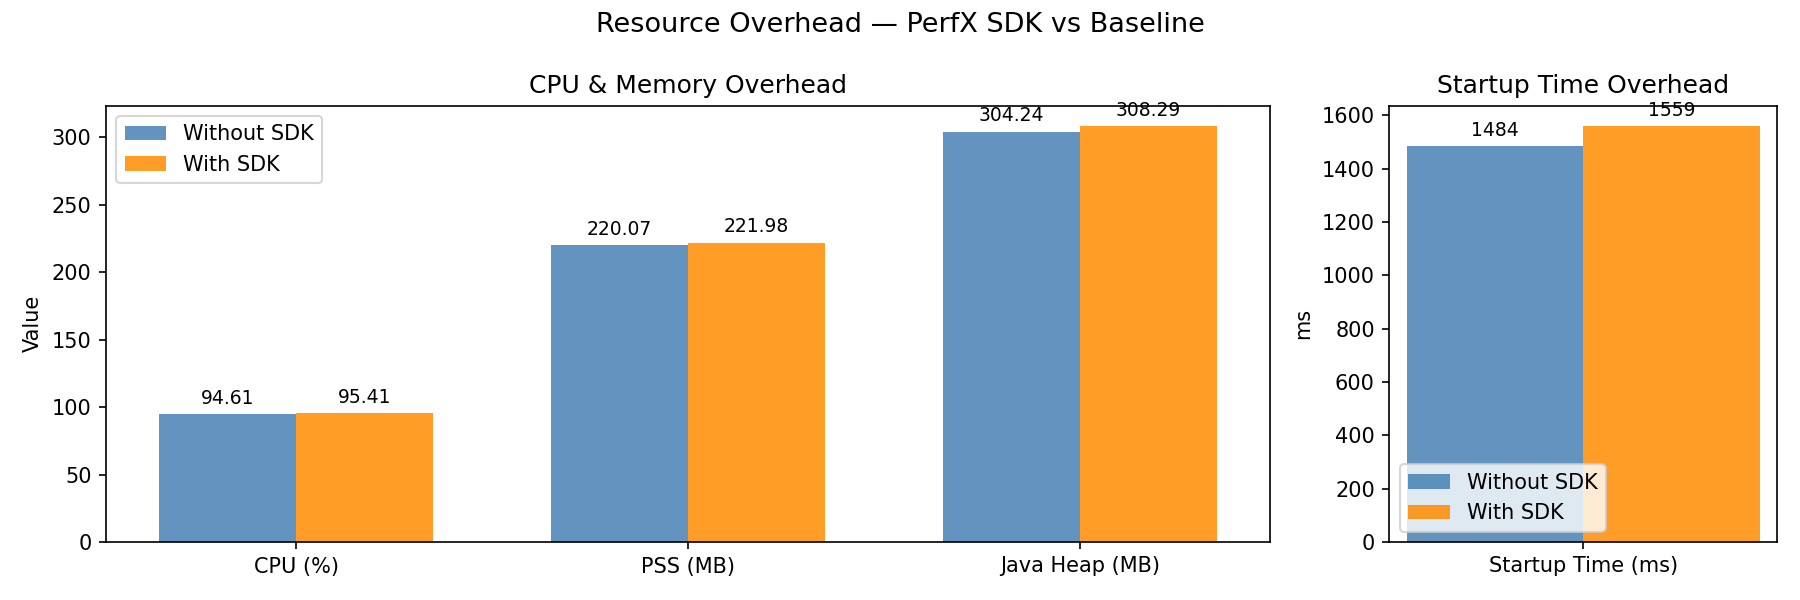
\includegraphics[width=\textwidth]{figs/overhead_redmi.png}
        \caption{Xiaomi Redmi Note 9 Pro (Medium, physical)}
    \end{subfigure}
    \hfill
    \begin{subfigure}[b]{0.48\textwidth}
        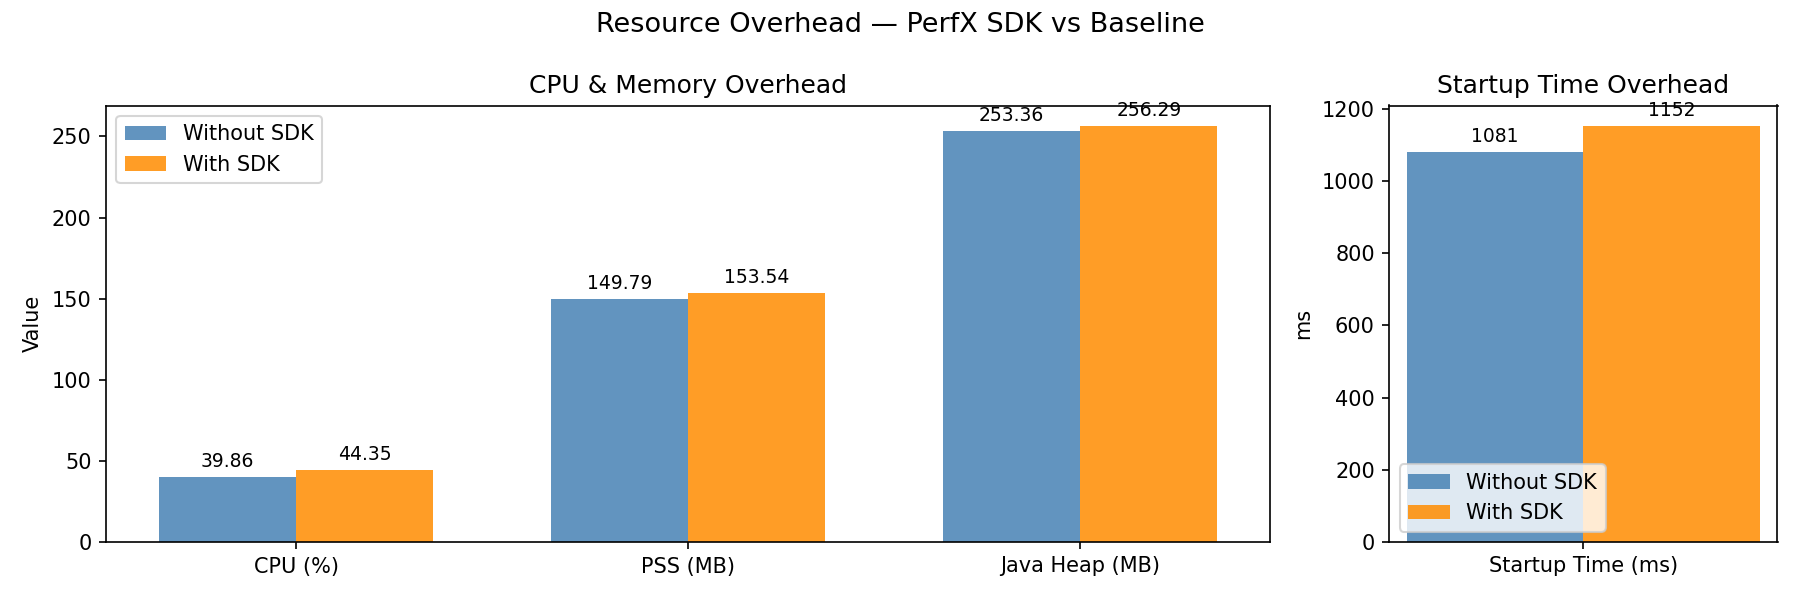
\includegraphics[width=\textwidth]{figs/overhead_low.png}
        \caption{Emulator — Low cohort}
    \end{subfigure}

    \vspace{0.5em}

    \begin{subfigure}[b]{0.48\textwidth}
        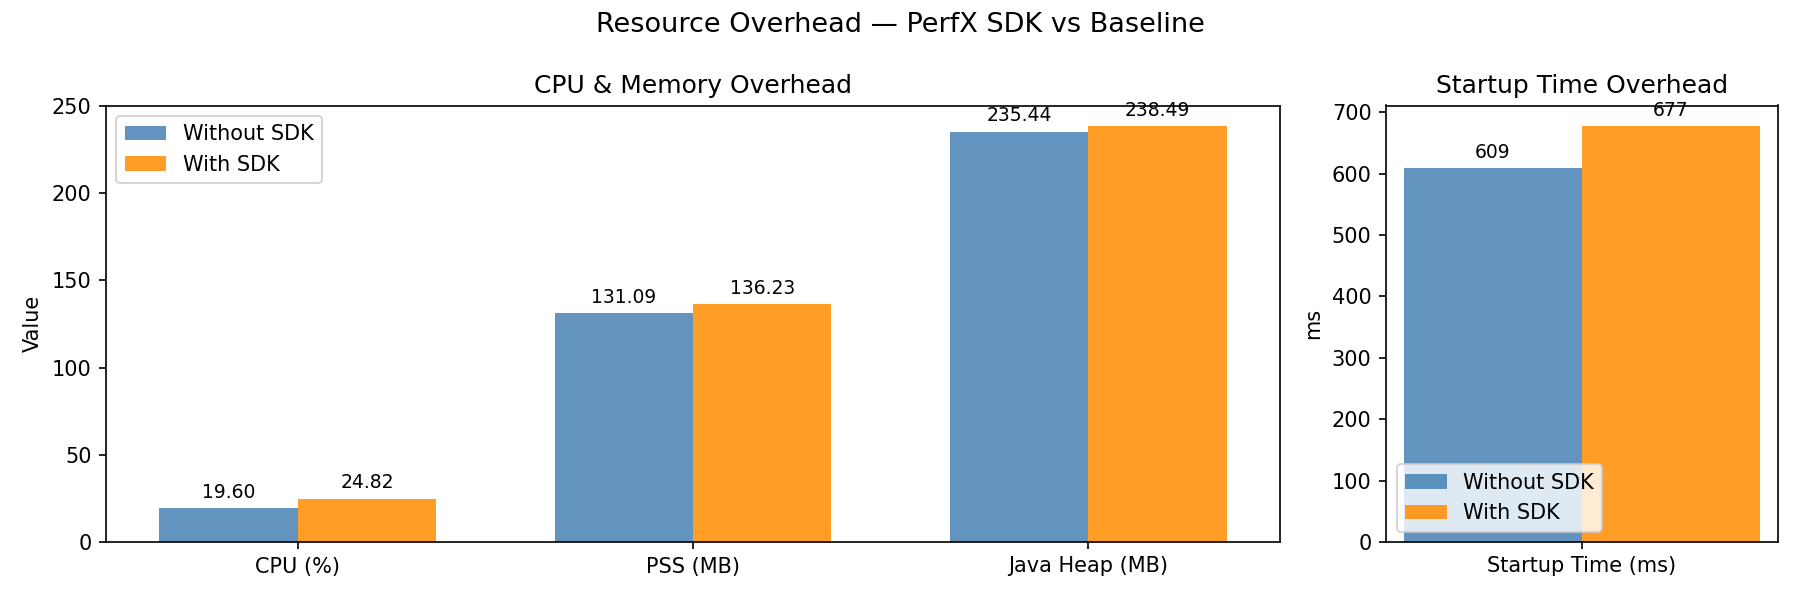
\includegraphics[width=\textwidth]{figs/overhead_medium.png}
        \caption{Emulator — Medium cohort}
    \end{subfigure}
    \hfill
    \begin{subfigure}[b]{0.48\textwidth}
        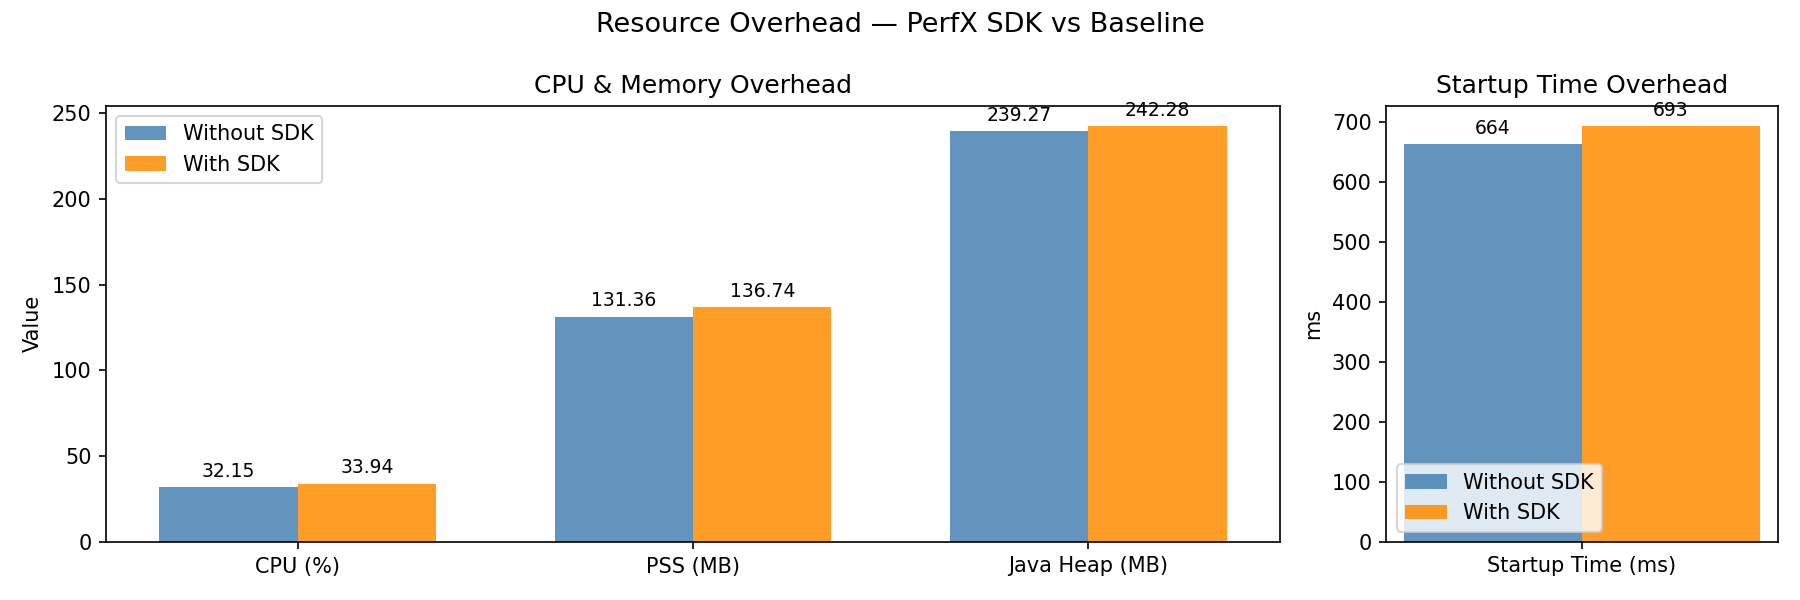
\includegraphics[width=\textwidth]{figs/overhead_high.png}
        \caption{Emulator — High cohort}
    \end{subfigure}
    \caption{SDK overhead charts for all four test devices. Each chart shows mean CPU usage, PSS memory, and cold-start time without and with the SDK enabled.}
    \label{fig:overhead_summary}
\end{figure}

The measured CPU overhead on the physical device is lower than the approximately 6~\% reported for the Panappticon tracing system~\cite{Panappticon}. Together with the consistent memory overhead and the moderate one-time cold-start cost, these results support the low-overhead requirement defined in Section~\ref{sec:req} across all tested device cohorts.

\section{Metric Validity}
\label{sec:eval_accuracy}

Each metric is collected using the authoritative Android platform API for that measurement, as described in Section~\ref{sec:sdk_impl}. For this reason, a separate metric-accuracy experiment against external reference tools was not carried out: it would compare one platform API against another rather than testing the SDK itself, and any observed deviation would reflect differences in sampling granularity or timing between tools, not errors introduced by the SDK. The correctness of the SDK's measurements therefore rests on the correctness of the Android platform APIs, which are maintained by the Android Open Source Project and used in production profiling tooling. The evaluation accordingly focuses on detection accuracy (Section~\ref{sec:eval_regression}), not on re-measuring the platform APIs.

\section{Regression Detection Evaluation}
\label{sec:eval_regression}



This section evaluates the ability of the regression detection pipeline to correctly identify performance regressions and to produce no alerts in their absence. Two builds of the demo application were compared for each experiment: a baseline build with no regression and a second build with a known regression introduced, as described in Section~\ref{sec:eval_setup}.

\subsection{Experiment Setup}

Each build was launched on the target device and run for one minute, during which the SDK forwarded metric samples to the backend. The detector then compared the P95 of each metric between the two version codes, grouped by metric, screen, and device cohort. A regression was flagged when the relative P95 shift exceeded 15\%.

\textbf{Experiment matrix.} Three regression types (CPU load, memory leak, UI thread blocking) were evaluated at three intensity levels (low, medium, high) on three device cohorts (Low, Medium, High), giving 27 experiment cells in total.

\textbf{Control runs.} Five runs per cohort with no injected regression were carried out to measure the false-positive rate. These results are reported in Section~\ref{sec:eval_threshold}.

\subsection{Regression Injection}

A CPU regression was simulated by launching one or more background coroutines on \texttt{Dispatchers.Default}, each running a tight prime-number sieve in a loop. The number of concurrent workers was one, two, and four for low, medium, and high intensity. A 10\,ms cooperative yield was added to each iteration so that the SDK upload coroutines were not completely starved.

A memory regression was simulated by allocating 256\,KB byte arrays at regular intervals and retaining all of them in a list, preventing the garbage collector from reclaiming them. The allocation rate was one, two, and three chunks every 200\,ms for low, medium, and high intensity.

A UI thread regression was simulated by calling \texttt{Thread.sleep()} inside a \texttt{withFrameMillis} callback on the main thread, blocking it for a fixed duration on every rendered frame. The block durations were 15\,ms, 40\,ms, and 90\,ms per frame for low, medium, and high intensity respectively.

\subsection{Detection of Injected Regressions}
\label{sec:eval_e1}

Table~\ref{tab:eval_regression} reports the baseline and current P95 values, the relative P95 shift, and the detection outcome for each of the 27 cells. The detection rate aggregated across all 30 runs is shown in Figure~\ref{fig:e1_detection_rate}.

\begin{table}[htbp]
    \centering
    \small
    \caption{P95 Shift and Detection Outcome for the Injected Regressions (Release-Pair Comparison, 15\% Threshold)}
    \label{tab:eval_regression}
    \begin{tabular}{llrrrrl}
        \toprule
        Metric          & Intensity & Cohort & Baseline & Current & $\Delta$ (\%) & Detected         \\
        \midrule
        CPU usage (\%)  & Low       & Low    & 6.29     & 7.15    & 13.6          & No               \\
        CPU usage (\%)  & Low       & Medium & 8.31     & 9.55    & 15.1          & Partial (2 of 4) \\
        CPU usage (\%)  & Low       & High   & 10.22    & 12.97   & 27.0          & Yes              \\
        CPU usage (\%)  & Medium    & Low    & 9.49     & 17.20   & 81.3          & Yes              \\
        CPU usage (\%)  & Medium    & Medium & 3.79     & 5.16    & 36.0          & Yes              \\
        CPU usage (\%)  & Medium    & High   & 10.18    & 20.24   & 98.8          & Yes              \\
        CPU usage (\%)  & High      & Low    & 9.40     & 137.53  & 1363.0        & Yes              \\
        CPU usage (\%)  & High      & Medium & 9.98     & 132.77  & 1230.3        & Yes              \\
        CPU usage (\%)  & High      & High   & 10.56    & 170.06  & 1510.8        & Yes              \\
        \addlinespace
        Memory (MB)     & Low       & Low    & 72.88    & 87.99   & 20.7          & Yes              \\
        Memory (MB)     & Low       & Medium & 71.04    & 86.19   & 21.3          & Yes              \\
        Memory (MB)     & Low       & High   & 68.94    & 84.13   & 22.0          & Yes              \\
        Memory (MB)     & Medium    & Low    & 72.86    & 152.23  & 108.9         & Yes              \\
        Memory (MB)     & Medium    & Medium & 71.12    & 150.66  & 111.8         & Yes              \\
        Memory (MB)     & Medium    & High   & 68.96    & 148.90  & 115.9         & Yes              \\
        Memory (MB)     & High      & Low    & 72.83    & 202.09  & 177.5         & Yes              \\
        Memory (MB)     & High      & Medium & 71.63    & 200.41  & 179.8         & Yes              \\
        Memory (MB)     & High      & High   & 69.09    & 198.35  & 187.1         & Yes              \\
        \addlinespace
        Frame time (ms) & Low       & Low    & 16.67    & 25.83   & 55.0          & Yes              \\
        Frame time (ms) & Low       & Medium & 16.67    & 20.00   & 20.0          & Yes              \\
        Frame time (ms) & Low       & High   & 19.23    & 29.41   & 52.9          & Yes              \\
        Frame time (ms) & Medium    & Low    & 16.67    & 50.00   & 200.0         & Yes              \\
        Frame time (ms) & Medium    & Medium & 16.67    & 45.46   & 172.7         & Yes              \\
        Frame time (ms) & Medium    & High   & 17.26    & 51.67   & 199.3         & Yes              \\
        Frame time (ms) & High      & Low    & 16.67    & 100.00  & 500.0         & Yes              \\
        Frame time (ms) & High      & Medium & 16.67    & 100.00  & 500.0         & Yes              \\
        Frame time (ms) & High      & High   & 17.27    & 106.67  & 517.5         & Yes              \\
        \bottomrule
    \end{tabular}
\end{table}

\begin{figure}[H]
    \centering
    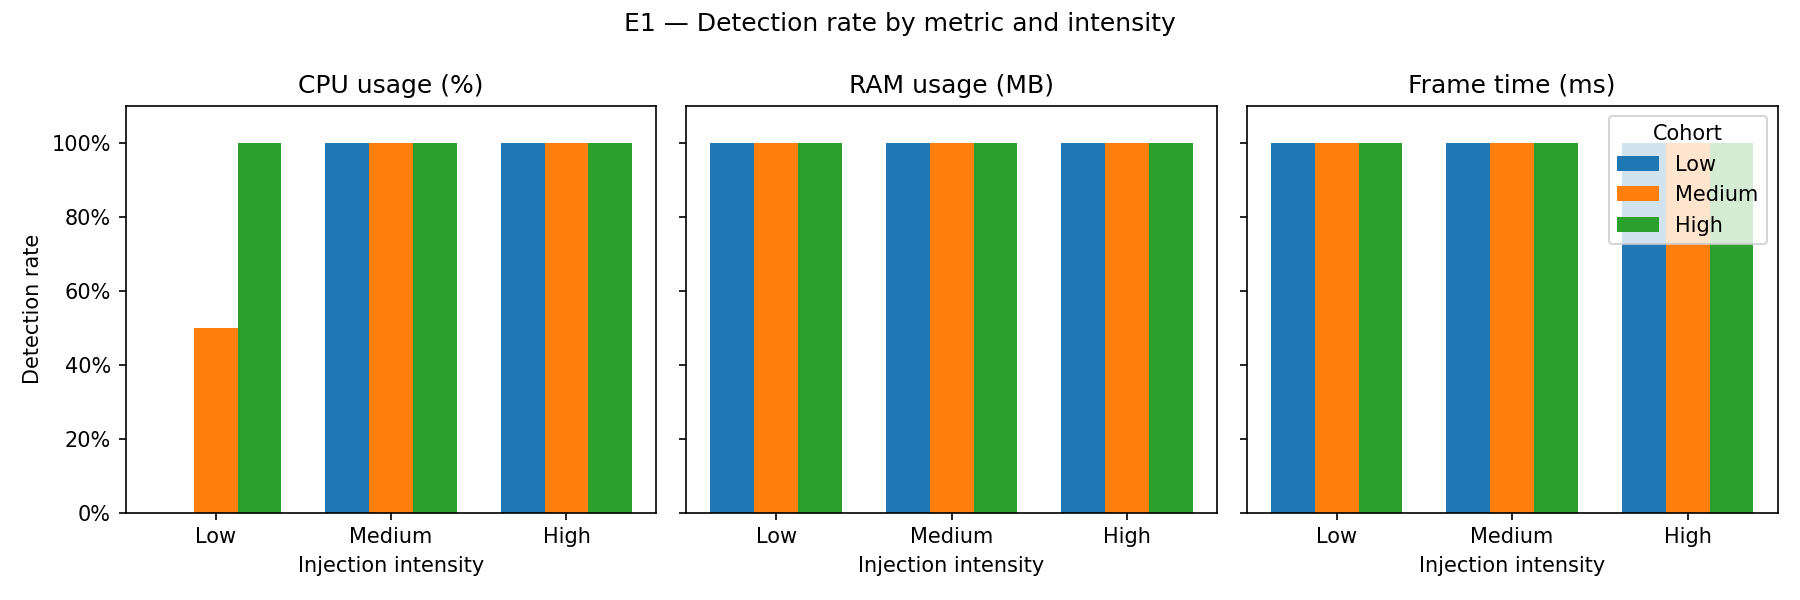
\includegraphics[width=\textwidth]{figs/e1_detection_rate.png}
    \caption{Detection rate by metric, injection intensity, and device cohort. Each bar shows the fraction of runs in that cell that the detector flagged as a regression at the 15\% threshold.}
    \label{fig:e1_detection_rate}
\end{figure}

The detector flagged 27 of the 30 runs (90\%). All 27 cells with intensity at medium or high were detected on every cohort, including the very large P95 shifts produced by the high-intensity injections. The three missed runs all fall into the low-intensity CPU configuration: the Low-cohort run produced a P95 shift of 13.6\%, just below the 15\% threshold, and the Medium-cohort cell was at the threshold border, with two of four runs detected and two not. The High cohort still detected the same configuration at a P95 shift of 27.0\%, because the baseline CPU usage on that emulator was slightly higher and the same injection produced a larger relative shift.

The remaining 24 cells were detected with margin: the smallest relative shift among detected cells was 20.0\% (UI low on Medium), and most cells exceeded the threshold by an order of magnitude. The detector therefore reliably flags injections whose relative effect on the P95 value is at least roughly twice the configured threshold and behaves less reliably for injections whose effect is close to or below the threshold.

\subsection{Threshold Sensitivity}
\label{sec:eval_threshold}

The 15\% threshold used above is one configuration choice. To show the trade-off between detection rate and false positives across choices, the same 30 injected runs and the 15 control runs were reanalysed at thresholds from 5\% to 50\%. The true-positive rate (TPR) was computed on the 30 injected runs and the false-positive rate (FPR) on the 15 control runs. Table~\ref{tab:eval_threshold} reports the result at a few representative thresholds, and Figure~\ref{fig:e3_threshold_sweep} shows the full sweep.

\begin{table}[htbp]
    \centering
    \small
    \caption{Detector Quality vs.\ Regression Threshold}
    \label{tab:eval_threshold}
    \begin{tabular}{cccccc}
        \toprule
        Threshold & TPR  & FPR  & Precision & F1   & Comment                                \\
        \midrule
        0.05      & 1.00 & 0.13 & 0.95      & 0.98 & High recall, some false alerts         \\
        0.10      & 1.00 & 0.07 & 0.98      & 0.99 & Best F1 in the swept range             \\
        0.15      & 0.95 & 0.07 & 0.98      & 0.96 & Default threshold                      \\
        0.20      & 0.93 & 0.00 & 1.00      & 0.96 & First threshold with zero false alerts \\
        0.25      & 0.81 & 0.00 & 1.00      & 0.89 & Misses borderline low-intensity cells  \\
        0.30      & 0.76 & 0.00 & 1.00      & 0.86 & Conservative, prefers precision        \\
        \bottomrule
    \end{tabular}
\end{table}

\begin{figure}[H]
    \centering
    
\includegraphics[width=0.85\textwidth]{figs/e3_threshold_sweep.png}
    \caption{Detector quality as a function of the relative-shift threshold. TPR and FPR are computed on the 30 injected runs and 15 control runs respectively. The vertical dashed line marks the default threshold of 15\%.}
    \label{fig:e3_threshold_sweep}
\end{figure}

The sweep shows two regions. Below 0.15 the detector finds every injected regression but also reports a small number of false alerts on the control runs: one or two false positives out of 15. At and above 0.20 the false-positive count drops to zero but recall falls as well, because the low-intensity CPU cells near the threshold are now missed.

The 15\% default sits at the boundary between these two regions. It keeps recall above 95\% while accepting one false positive in 15 control runs (6.7\% FPR) on the data collected in this evaluation. A 0.20 threshold trades roughly two percentage points of recall for zero false alerts on this dataset. The choice between the two depends on the operating preference: a system tuned for catching as many regressions as possible should use 0.15 or lower, while a system tuned to minimise developer alert fatigue should use 0.20.

\section{Discussion of Results}
\label{sec:eval_discussion}

This section interprets the results in relation to the three research questions defined in Chapter~\ref{chap:intro}.

The first research question asks how Android application performance can be monitored continuously with low runtime overhead. The results in Section~\ref{sec:eval_overhead} show that enabling the SDK added at most 5.2 percentage points of CPU usage, 5.4~MB of memory, and 75~ms of cold-start time across all tested devices. These costs are small enough that an end user is unlikely to perceive them, and are consistent with the background sampling, two-tier buffering, and batched transmission design described in Chapter~\ref{chap:impl}.

The second research question asks how performance regression introduced by application updates can be detected automatically. The pipeline groups metric samples by version code, metric, screen, and device cohort, applies a maturity gate, and then flags a regression when the relative P95 shift between two consecutive releases exceeds the configured threshold. This approach requires no manual labelling and no per-metric threshold tuning, and it runs continuously against incoming production data.

The third research question asks how accurate the proposed system is in detecting performance regressions. The pipeline detected 27 of 30 injected runs (90\%) across three regression types, three intensity levels, and three device cohorts. At the default 15\% threshold, one false alert was produced in 15 control runs (FPR $\approx 7\%$). Raising the threshold to 20\% eliminates false alerts at the cost of roughly two percentage points of recall, as shown in Section~\ref{sec:eval_threshold}. The three missed detections all fall in the low-intensity CPU configuration, where the P95 shift sits at or just below the threshold.

\section{Limitations}
\label{sec:eval_limitations}

The evaluation has several limitations.

First, the system was not deployed to real users. Overhead and detection quality were measured on a small fixed set of devices running one usage scenario, which does not capture the variety of real-world usage.

Second, emulators do not fully replicate the hardware behaviour of physical devices, so the emulator results for CPU and memory should be treated as indicative rather than conclusive.

Third, the device cohort is assigned using a simple rule based only on total RAM and CPU core count. Two devices with the same RAM and the same number of cores can still differ in real performance because of their chipset, GPU, or thermal behaviour, so this rule may place a device in the wrong cohort and weaken the cohort-based comparison.
